\section{Introduction}

\subsubsection{Importance of analysing watch time.} YouTube starts to stress on watch time rather than view number.

We borrow the idea of two-step process from \cite{krumme2012quantifying}, the decision to click and decision to watch are two independent actions. The amount of time audience spend on the product reflects the intrinsic quality.

\subsubsection{A metric to quantify video quality.} Quality of video is a loose defined concept. We use video watch percentage as a proxy to measure video quality.

\subsubsection{Cold-start predicting watch percentage}

%----------------------------------------------------------------------------------------

\section{Related work}

\subsubsection{YouTube watching behavior} Video watch time associates with popularity metrics (e.g., view count, the number of comments and shares) and user reaction (e.g., sentiment polarity of comments, the number of likes and dislikes) collectively \cite{park2016data}. However, their observations base on a prior observation period, while our focus is different, without observing an early reaction from video audiences, can we predict watch percentage from a cold start setting up? Or can we classify a bunch of quality videos?

\subsubsection{Model of predicting future view count} Peeking strategy and \textit{ex-ante} prediction \cite{martin2016exploring}.

%----------------------------------------------------------------------------------------

\section{Data and measurement}

In order to study YouTube watching behavior, we built a tool to collect video watching statistics on a daily basis. In this section, we first introduce a large dataset that contains rich features from nearly 20 million YouTube videos, then provide intuitive measurements on YouTube watching behavior.

\subsection{Data Collection}

\noindent\textbf{Random Videos:} To obtain a sample of YouTube videos, we used Twitter appearance as a selecting policy. With the help of Twitter Streaming API, first we crawled 202 million tweets that contained "YouTube" keyword over two months period, from July 1st, 2016 to August 30th, 2016. We then parsed the associated shortened URL and only considered tweets that linked to a genuine YouTube video page. Out of these, 36 million video IDs were identified. Finally, we used YouTube Data API and YTCrawl tool \cite{yu2015lifecyle} to acquire video metadata and daily viewing statistics respectively. After accounting the effects of Twitter sampling, video attrition and private statistics, our Random Videos resulted in a total set of nearly 20 million YouTube videos. Furthermore, we grouped these random videos by category to constitute Random Music dataset, Random News dataset, et cetera. We regarded Random Videos as an approximation of overall YouTube videos.

The most two prominent and valuable statistics of this dataset are daily watch time \textit{WatchT} and daily view count \textit{View}. Upon those, we can derive portion of watching \textit{WatchP} that an average user spends per view at a daily granularity by performing a pairwise division \textit{WatchT}/\textit{View}/duration. We user this series data \textit{WatchP} to reveal watching behavior temporal trend (see section xx). Besides, we extract \textit{WatchP@180} as \textit{WatchT@180}/\textit{View@180}/duration to approximate the intrinsic property.

\noindent\textbf{Quality Videos:} The Quality Videos dataset consists of two parts, VEVO dataset and Top News dataset. VEVO dataset contains videos from all verified VEVO accounts on YouTube platform; Top News dataset features top 100 most viewed News channels, as reported by external source \footnote{https://vidstatsx.com/youtube-top-100-most-viewed-news-politics}. The number of videos and corresponding statistics in each dataset can be found in Table~\ref{table:1}.

\begin{table*}
  \caption{Overview of datasets}
  \label{table:1}
  \begin{tabular}{ccccc}
    \toprule
    Dataset & \#Videos & \#Channels & \#Avg Views & \#Avg Watch Time/View \\
    \midrule
    Random Videos & 19,464,997 &  & \\ 
    Random Music & 2,179,330 & 649,895 & \\ 
    VEVO & 72,488 & 14,342 & \\
    Random News & 1,079,149 & 105,853 & \\
    Top News & 29,732 & 91 & \\
  \bottomrule
\end{tabular}
\end{table*}

\subsection{Blockbuster consumes more time}

Long before the creatiion of watch time concept, number of views works as the golden metrics to evaluate success of YouTube video, meanwhile serve as income for content producer. Viewing behavior has also been treated as a popular field in academic world, researchers explore many models to explain and predict viewership. However, there are various ways to boost viewership without what so called, "organic growth", such as utilize marketing company for paid views or use click farm, even spread spam email or tweets on other social media. In this sense, YouTube converts to focus on another more engagement metrics, embed it into their recommender systems to help user discover better content, which is watch time.

A question could be how different watch time and view count express? Bear this in mind, we investigate the relationship between watch time and view count.

First, we examine ranking list sorted by view and watch by using co-occurrence and Kendall's tau as our evaluation metrics. Out of our 20million random dataset, we rank videos by view@180 and watch@180, then construct top list with n between 100 and 10,000 at step of 100. Figure 1(a) illustrates more than 30\% of top videos disagree on those two lists and their order shows a large disagreement. More than 70\% of concordant have been fliped. This experiment shows a very different result if we consider ranking by view count and watch time.

Figure 1(b) tells a "Winner takes all" story. Interestingly, we observe a positive relationship between view count and average watch time. The more views a view receives, the more time audience spend on it. This corresponds with "Rich gets richer" theory, and here the popular videos not just take more clicks, they consume more time.

\begin{figure}
\subfloat[Ranking comparison]{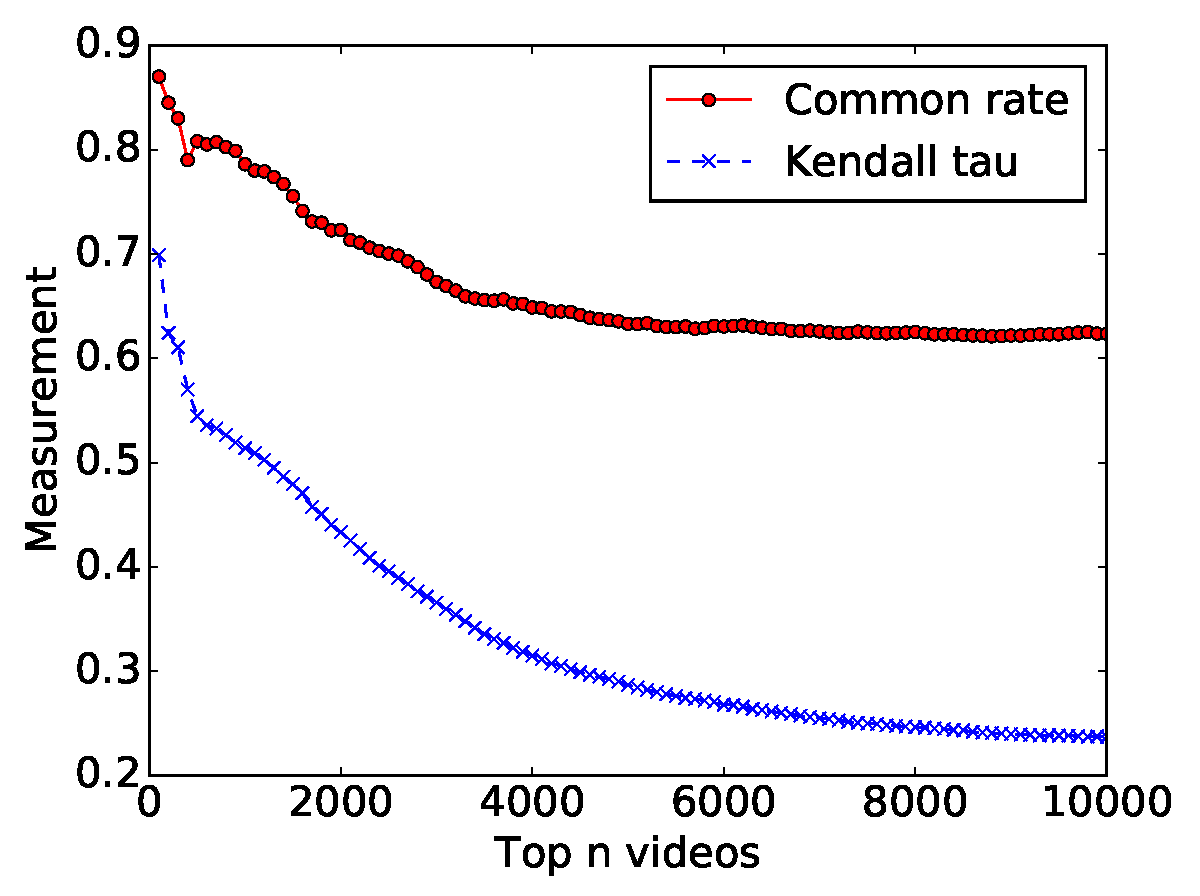
\includegraphics[width=0.25\textwidth]{image/rank_by_view_and_watch.pdf}}
\subfloat[View count vs. avg watch time]{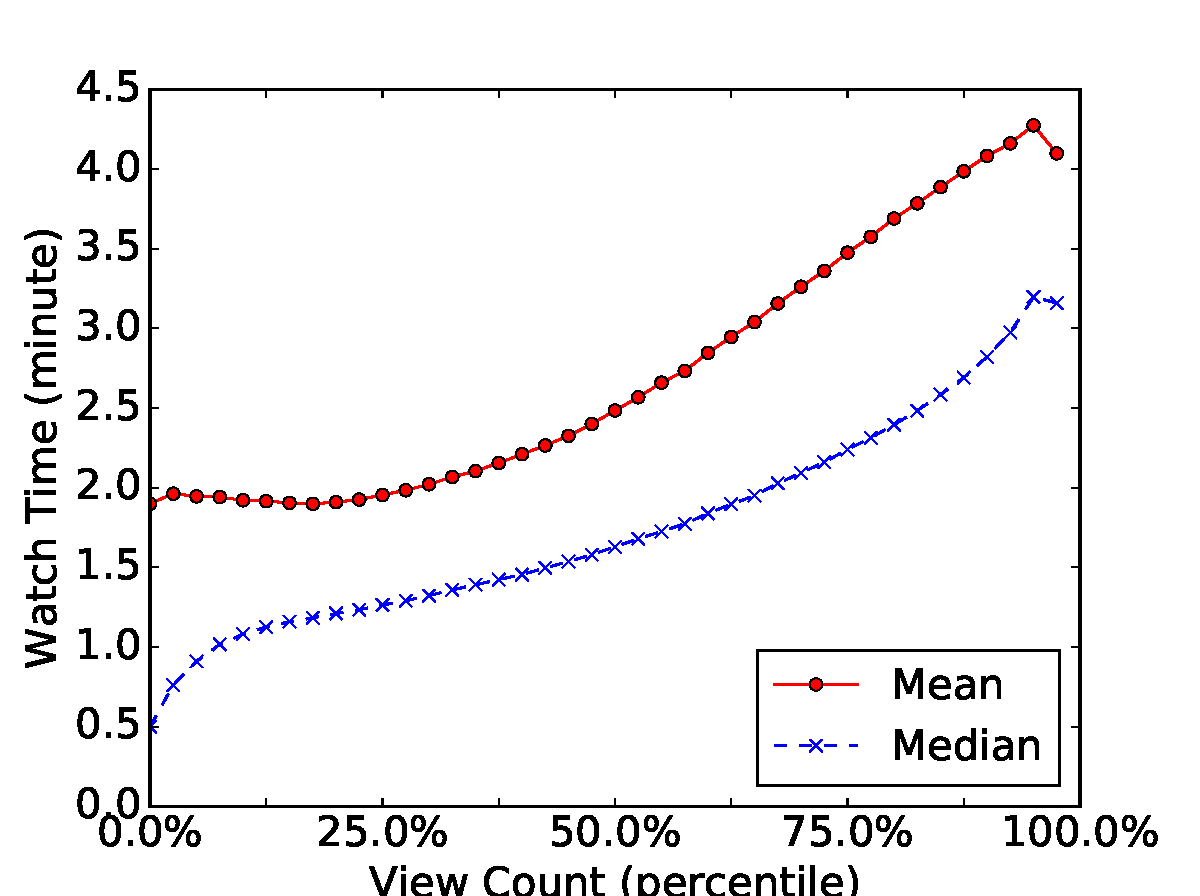
\includegraphics[width=0.25\textwidth]{image/watch_against_view_overall.pdf}}
\caption{View count and watch time. (a) The ranking results given by those 2 metrics vary significant. (b) Users not just click more on blockbuster, they also spend more time per view on blockbuster.}
\end{figure}

\subsection{Proxy of video quality}

Through the fitting procedure in section 3.4, we convert a watch percentage time series into 2 variables, initial watch percentage \textit{initial wp} and decay rate \textit{R}. Next we are interested to see whether those variable can be a proxy of video quality, taking duration and category as control variable. Video quality is a loose defined concept. It's a mix of production quality, content topic and channel profile.

We leverage external resource to validate video quality, create a VEVO music dataset and Top News dataset as stated in Table 1. We use the hypothesis that VEVO artists come from professional background thus having a better video quality, so does news video that comes from professional news agency. Next we compare the watch percentage from quality dataset to random dataset, since we know watch percentage is heavily impacted by video duration, thus we take duration as a control variable. As expected, quality videos sit on the top of random videos, this validates our hypothesis quality videos have a higher watch percentage than random videos.

\begin{figure}
\centering
\subfloat[Overall]{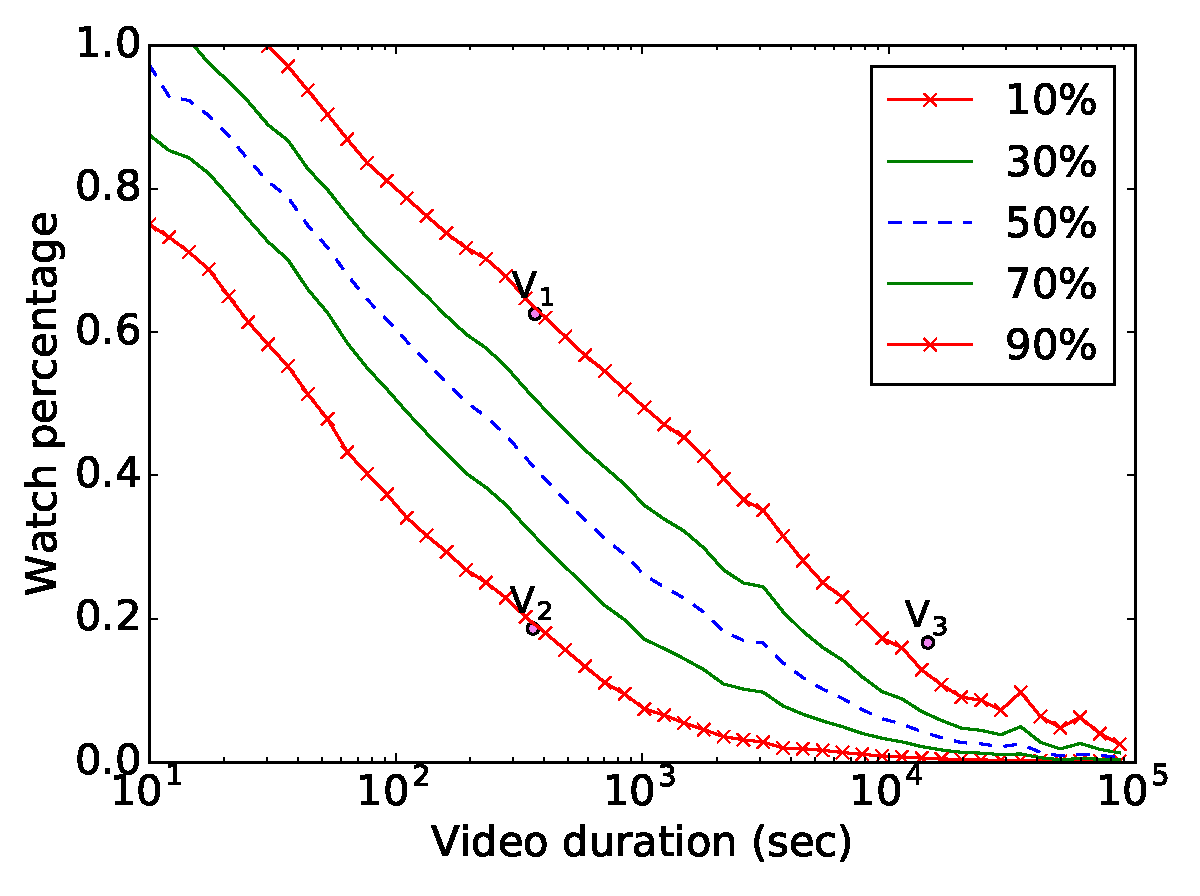
\includegraphics[width=0.5\textwidth]{image/wp_vs_duration_overall.pdf}}

\subfloat[Music]{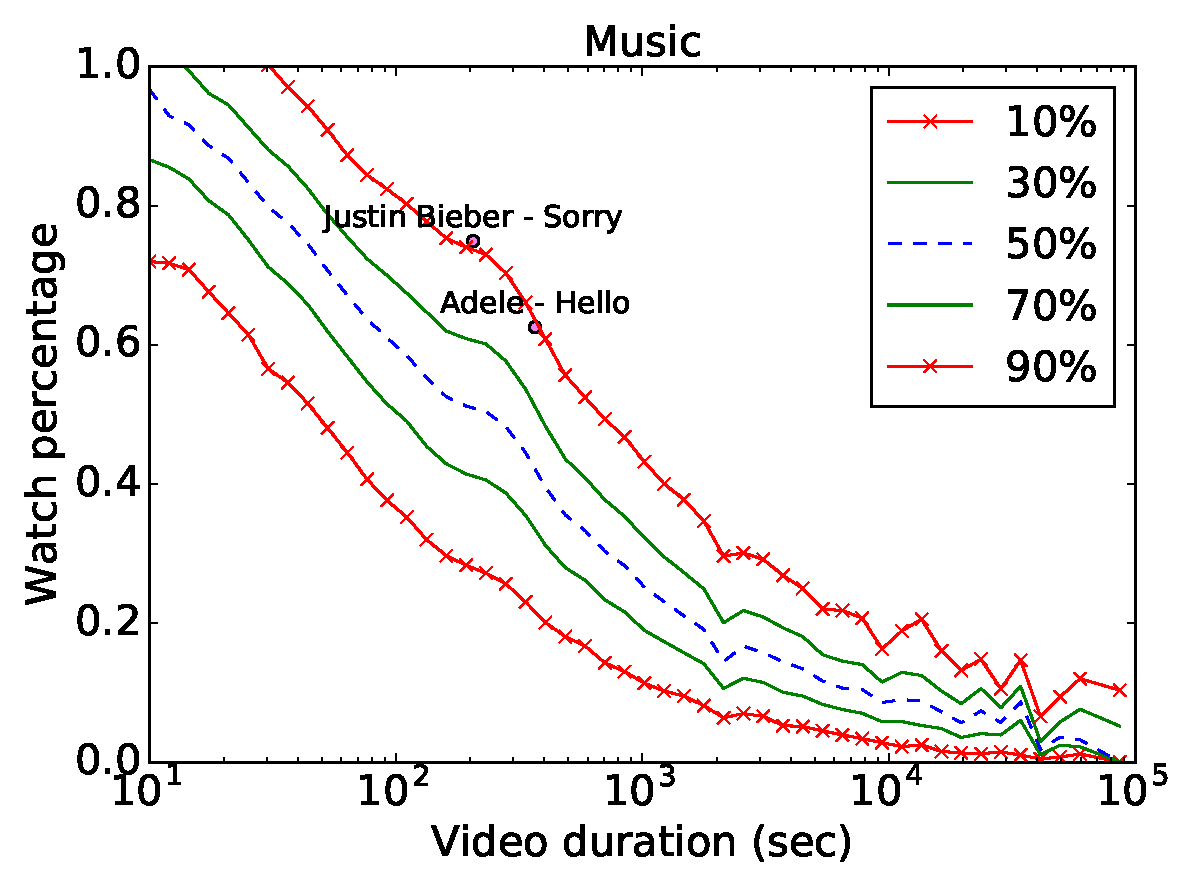
\includegraphics[width=0.25\textwidth]{image/wp_vs_duration_music.pdf}}
\subfloat[News]{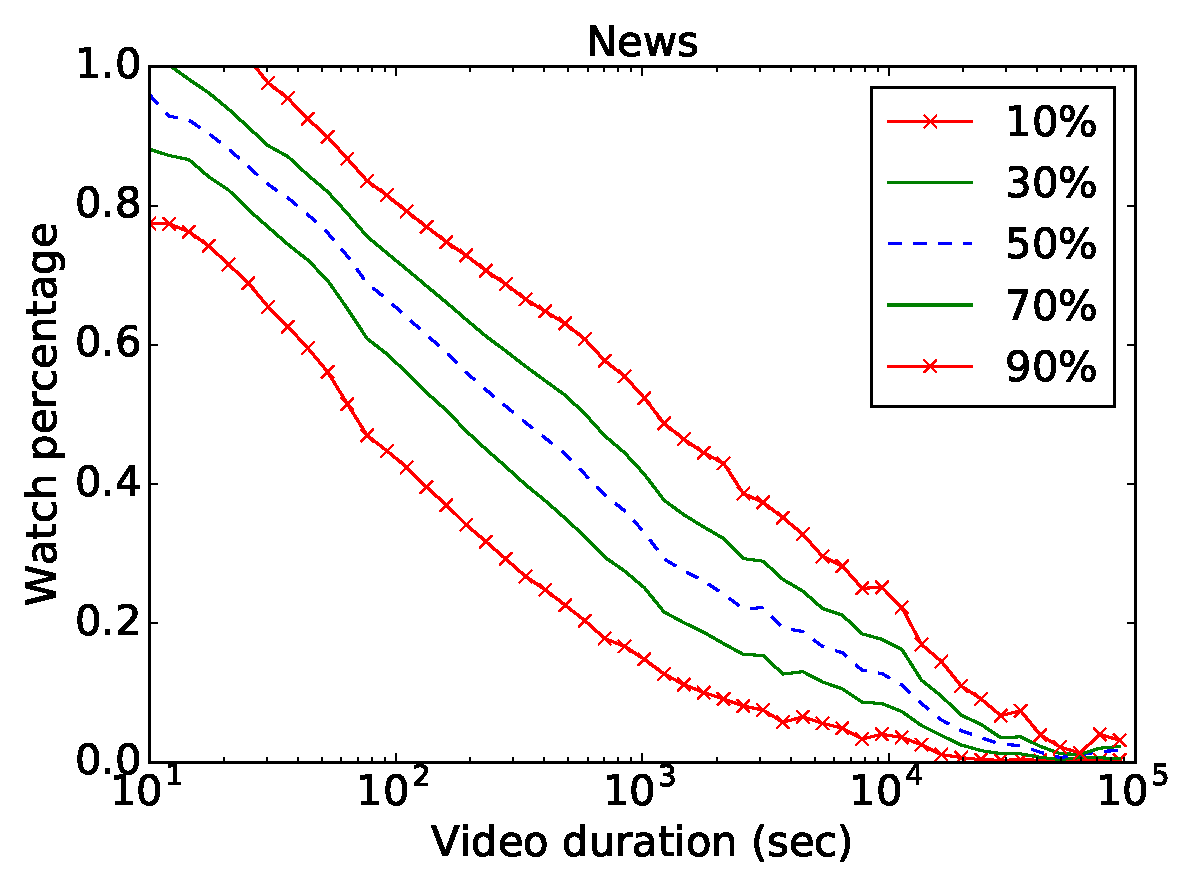
\includegraphics[width=0.25\textwidth]{image/wp_vs_duration_news.pdf}}
\caption{Watch percentage and duration. (a) parameters come from 19M YouTube videos. 3 Music videos are shown on panel to depict difference. v1 (id \textit{YQHsXMglC9A}): a quality short video that attract clicks and attentions; v2 (id \textit{NzpOcMo6280}): even though v2 also exhibits a strong capability to attract clicks (3,930,180 clicks) but people intent to leave quickly, we name it as junk video; v3 (id \textit{brrn4vOwdDM}): although people only watch 0.2 of it, but since its longer duration, we still consider it as a quality video.}
\end{figure}

\subsection{Watch percentage temporal pattern}

Many works have shown that temporal view count could be explained by a relaxed exponential decay \cite{(R.Crane and D.Sornette, viral videos short paper)}, it's natural to ask how watch percentage evolves over time. Even though watch percentage is a value that bounded from 0 to 1, we still find exponential decay explain the best among the other two methods, i.e, linear regression, or consider watch percentage to be a constant irrelevant to video age. The fitting result can be found in fig 1.

In this section, we try to avoid that watch percentage varies too much resulting from insufficient views, therefore we preprocess our Random dataset to identify a group of videos that attract enough attentions during its lifecycle. We adopted a selection criteria that video must have at least 80 day with daily view over 20 in the first 120 days, this filter ends up with 1.9 million videos.

Next we try to group those active videos by watch percentage trend. We select a changing threshold of 10\%, which requires the change of watch percentage in the 120 days less than threshold, If the change is over threshold, then we consider them as growth videos, to present a more involved watching behavior as the video gets older. If the change goes down below the threshold, we consider people lose interests as they get older. For videos fall inbetween, we consider them as memoryless videos as the watch behavior on them are consistent throughout the whole lifecycle. A demonstration of those 3 types can be found in fig 2.

\begin{figure}
    \centering
    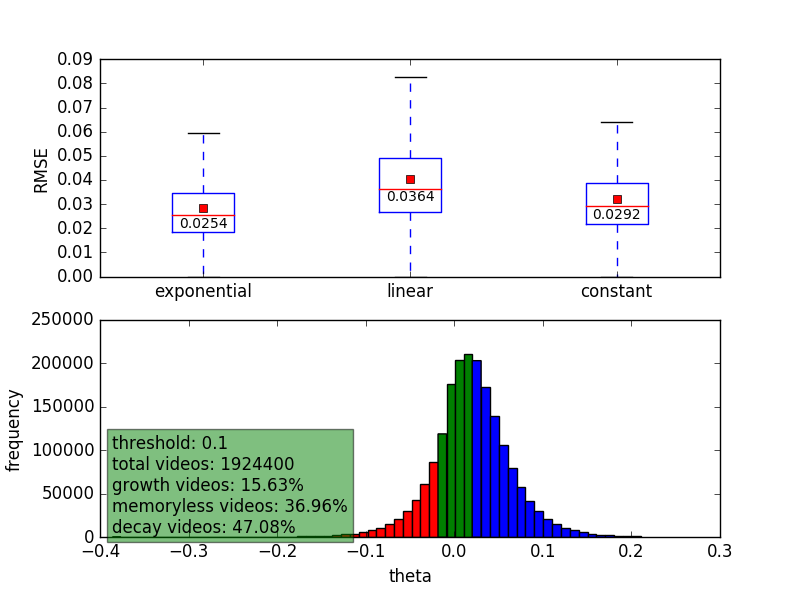
\includegraphics[scale=0.45]{image/wp_rmse_comp_and_theta_dist.png}
    \caption{Temporal watch percentage fitting}
\end{figure}

\section{Burst view and engagement}

We are also interested in whether a burst of views would harm the engagement. It can result from various motivations, such as YouTube recommender system delivers content to a majority of audience, but the video can be of great general interest or niche to specific group; or channel owner uses promotion to get instant view count and in this situation, they are probably low quality views. In order to answer this question, first we need to identify view burst, then determine the causailty from bursty view to watch percentage.

We identify view burst as variable \textit{b} Vi/avg(sum(Vi-7 to Vi-1)), the ratio of view on current day upon average of previous seven days. The number of bursts relates to the value of \textit{b}. As \textit{b} goes up, the number of viewing burst inclines as shown in Fig 4.

We find that only a few videos could enjoy the spread of viewing, and those videos can embrace a revive from public attention. However for most videos, a sudden increase on views is likely to drag down watch percentage.

%----------------------------------------------------------------------------------------

\section{Cold start watch behavior prediction}

\subsection{Classify Quality Videos}
How well can this model with a floating quality threshold?

input: a new video, with metadata only (video features, user vector)

output: is this a quality video? (appear above the top x\% of duration percentile plot)

method: classification task; category, duration as control variable.

setup: 

\subsection{Predict Watch Percentage}
input: a new video, with metadata only (video features, user vector)

output: what's the watch percentage by day 30? performance matrix to select features

method: regression task; category, duration as control variable.

setup: 

%----------------------------------------------------------------------------------------

\section{Integrate with HIP: Predict future watch time}
HIP model, learn a set of parameters to map dailyshare to dailywatch

Question: does this model work better with watch percentage plugged in?

input: a new video, with observed dailyshare, dailywatch, daily watch percentage

output: a line that fit video watch time in entire (120? 30?) lifecycle, explain the video quality.

method: HIP and modified HIP
%\end{document}  % This is where a 'short' article might terminate



\appendix
%Appendix A
\section{Appendix}

\subsection{View count and average watch time}

\begin{figure}
\subfloat[Music]{\includegraphics[width=0.25\textwidth]{image/watch_against_view_music.pdf}}
\subfloat[News]{\includegraphics[width=0.25\textwidth]{image/watch_against_view_news.pdf}}

\subfloat[Entertainment]{\includegraphics[width=0.25\textwidth]{image/watch_against_view_entertainment.pdf}}
\subfloat[Gaming]{\includegraphics[width=0.25\textwidth]{image/watch_against_view_gaming.pdf}}
\caption{Average watch time against View count.}
\end{figure}

%\begin{acks}
%  The authors would like to thank Dr. Yuhua Li for providing the
%  matlab code of  the \textit{BEPS} method. 
%
%  The authors would also like to thank the anonymous referees for
%  their valuable comments and helpful suggestions. The work is
%  supported by the \grantsponsor{GS501100001809}{National Natural
%    Science Foundation of
%    China}{http://dx.doi.org/10.13039/501100001809} under Grant
%  No.:~\grantnum{GS501100001809}{61273304}
%  and~\grantnum[http://www.nnsf.cn/youngscientsts]{GS501100001809}{Young
%    Scientsts' Support Program}.
%
%\end{acks}
